% Compile with latex to get .div output
% Then execute dvisvgm to convert .div to .svg, use --no-fonts if fonts go wrong.
\documentclass[tikz]{standalone}
\usetikzlibrary{arrows.meta,positioning,automata}
\begin{document}
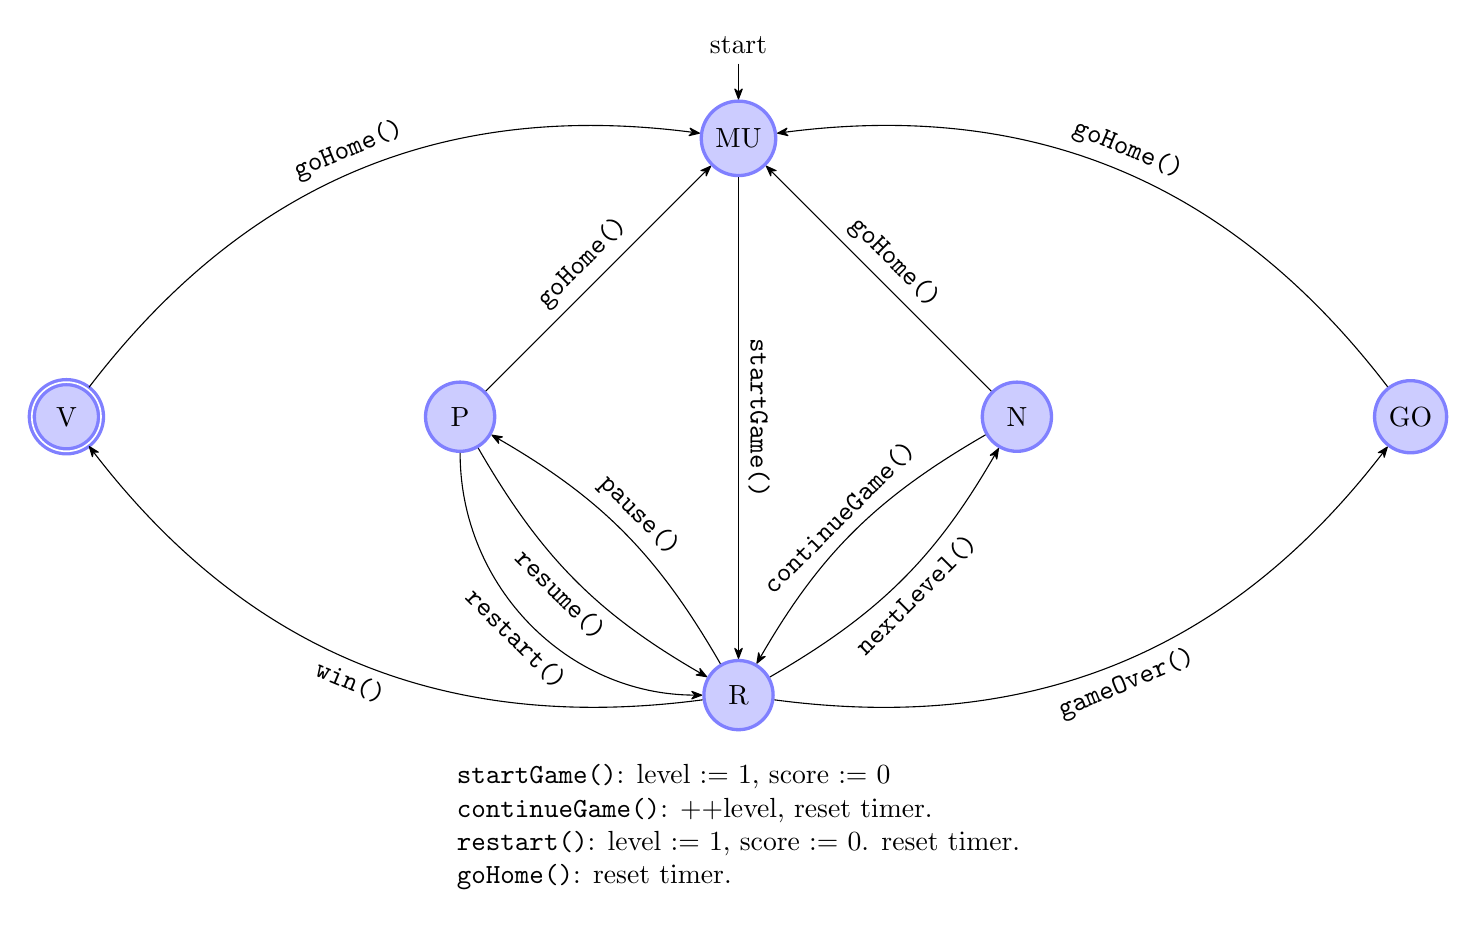
\begin{tikzpicture}[%
	node distance=5cm,on grid,>={Stealth[round]},
	every state/.style={draw=blue!50,very thick,fill=blue!20},
	initial where=above]

	\node[state,initial]	(MU)						{MU};
	\node[state]			(P)		[below left=of MU]	{P};
	\node[state]			(R)		[below right=of P]	{R};
	\node[state]			(N)		[below right=of MU]	{N};
	\node[state]			(GO)	[right=of N]		{GO};
	\node[state,accepting]	(V)		[left=of P]			{V};


	\path[->] (MU) edge					node	[sloped,above]	{\texttt{startGame()}}	
		(R);
	\path[->] (R)  edge	[bend right=15]	node	[sloped,above]	{\texttt{pause()}}			
		(P);
	\path[->] (P)  edge	[bend right=15]	node	[sloped,below]	{\texttt{resume()}}		
		(R);
	\path[->] (P)  edge	[bend right=45]	node	[sloped,below]	{\texttt{restart()}}		
		(R);
	\path[->] (P)  edge					node	[sloped,above]	{\texttt{goHome()}}		
		(MU);
	\path[->] (R)  edge	[bend left]		node	[sloped,below]	{\texttt{win()}}
		(V);
	\path[->] (V)  edge	[bend left]		node	[sloped,above]	{\texttt{goHome()}}
		(MU);
	\path[->] (R)  edge [bend right]	node	[sloped,below]	{\texttt{gameOver()}}
		(GO);
	\path[->] (GO) edge	[bend right]	node	[sloped,above]	{\texttt{goHome()}}
		(MU);
	\path[->] (N)  edge					node	[sloped,above]	{\texttt{goHome()}}
		(MU);
	\path[->] (N)  edge	[bend right=15]	node	[sloped,above]	{\texttt{continueGame()}}
		(R);
	\path[->] (R)  edge	[bend right=15]	node	[sloped,below]	{\texttt{nextLevel()}}
		(N);

	\node [anchor=top,below=3mm of R.south,align=left] {%
		\texttt{startGame()}: level := 1, score := 0\\
		\texttt{continueGame()}: ++level, reset timer.\\
		\texttt{restart()}: level := 1, score := 0. reset timer.\\
		\texttt{goHome()}: reset timer.
	};

\end{tikzpicture}
\end{document}